\documentclass[border=10pt]{standalone}
\usepackage{tikz}
\usetikzlibrary{decorations.pathmorphing,patterns}
\begin{document}
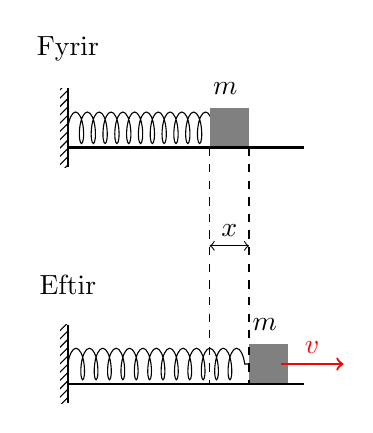
\begin{tikzpicture}
  \node(a) at (1,0) {};
  \node(g) at (1,0.5) {$m$};

  \node (t) at (-1,1) {Fyrir};

  \draw[decoration={aspect=0.3, segment length=1.5mm, amplitude=2mm,coil},decorate] (-1,0) -- (a);

  %\draw [->] (1,0.7) -- (0,0.7) node [midway, above]{$x$};

  \fill [pattern = north east lines] (-1,-0.5) rectangle (-1.1,0.5);
  \draw[thick] (-1,-0.5) -- (-1,0.5);
  \fill [gray] (0.8,-0.25) rectangle (1.3,0.25);

  \draw[thick] (-1,-0.25) -- (2,-0.25);
 % ----------
  \node(b) at (1.5,-3) {};
  \node(h) at (1.5,-2.5) {$m$};

  \node (s) at (-1,-2) {Eftir};
  \draw[decoration={aspect=0.3, segment length=1.7mm, amplitude=2mm,coil},decorate] (-1,-3) -- (b);

  %\draw [->] (1,0.7) -- (0,0.7) node [midway, above]{$x$};

  \fill [pattern = north east lines] (-1,-3.5) rectangle (-1.1,-2.5);
  \draw[thick] (-1,-3.5) -- (-1,-2.5);
  \fill [gray] (1.3,-3.25) rectangle (1.8,-2.75);

  \draw[thick] (-1,-3.25) -- (2,-3.25);

  %-----------

  \draw [dashed] (0.8,-0.25) -- (0.8,-3.25);
  \draw [dashed] (1.3, -0.25) -- (1.3,-3.25);

  \draw [<->] (0.8,-1.5) -- (1.3,-1.5) node [midway, above] {$x$};

  \draw[->, thick, red] (1.7,-3) -- (2.5,-3) node [midway, above] {$v$};


\end{tikzpicture}
\end{document}
